\cite{chabinUsingGraphGrammar2019,chabinGraphRewritingSystem2020} définit un cadre formel pour garantir la cohérence d'un graphe de connaissances \gls{rdf}.
L'approche introduit \gls{setup}, une méthode de maintenance des graphes \gls{rdf} qui repose sur la réécriture de graphes.
L'objectif est de maintenir le respect des contraintes d'intégrité du modèle \gls{rdfs} tel qu'expliqué dans \cite{flourisFormalFoundationsRDF2013}, \cite{halfeld-ferrariRDFUpdatesConstraints2017} ou encore \cite{chabinConsistentUpdatingDatabases2020}.
Les règles de la sémantique \gls{rdfs} sont formulées sous forme de règles logiques en utilisant les symboles de prédicats définis dans la table~\ref{table:update:soa:rdfs}.
Par exemple, la règle $(\forall x,y) CI(x,y) \to Cl(y)$ exprime que pour qu'un élément $x$ soit une instance de $y$, $y$ doit être une classe.
Pour modéliser ces règles de la sémantique, \cite{chabinUsingGraphGrammar2019} propose l'utilisation de la réécriture de graphes, illustrée par la figure~\ref{fig:gram_rule}.
Les règles ne peuvent être appliquées que si leur application préserve la cohérence du graphe.

\begin{figure}[htb]
    \centering
    \begin{subfigure}[b]{.3\textwidth}
        \centering
        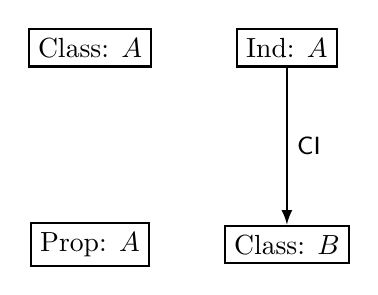
\begin{tikzpicture}[->, -latex, auto, node distance=2.5cm, thick, main node/.style={draw}]
            \node[main node] (1) {Class: $A$};
            \node[main node] (2) [below of=1] {Prop: $A$};
            \node[main node] (3) [right of=1] {Ind: $A$};
            \node[main node] (4) [right of=2] {Class: $B$};
            \path[every node/.style={font=\sffamily\small}]
            (3) edge node {CI} (4);
        \end{tikzpicture}
        \caption{\acs{nac}}
        \label{fig:gram_rule:nac}
    \end{subfigure}
    \begin{subfigure}[b]{.3\textwidth}
        \centering
        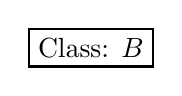
\begin{tikzpicture}[->, -latex, auto, node distance=2.5cm, thick, main node/.style={draw}]
            \node[main node] (2) {Class: $B$};
        \end{tikzpicture}
        \caption{\acs{lhs}}
        \label{fig:gram_rule:lhs}
    \end{subfigure}
    \begin{subfigure}[b]{.3\textwidth}
        \centering
        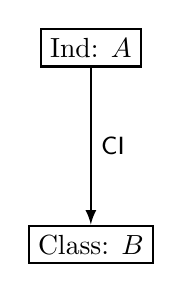
\begin{tikzpicture}[->, -latex, auto, node distance=2.5cm, thick, main node/.style={draw}]
            \node[main node] (1) {Class: $B$};
            \node[main node] (2) [above of=1] {Ind: $A$};
            \path[every node/.style={font=\sffamily\small}]
            (2) edge node {CI} (1);
        \end{tikzpicture}
        \caption{\acs{rhs}}
        \label{fig:gram_rule:rhs}
    \end{subfigure}
    \caption{Règle de réécriture simplifiée pour l'insertion du fait $CI(A,B)$}
    \label{fig:gram_rule}
\end{figure}

Les règles de réécriture sont des outils qui permettent de définir et de manipuler la structure des graphes en spécifiant comment le graphe doit évoluer selon certaines conditions.
Elles prennent la forme $\acs{lhs} \to \acs{rhs}$, où \gls{lhs} représente un motif dans le graphe et \gls{rhs} est le résultat de l'application de la règle.
Pour effectuer la réécriture, un morphisme est défini entre \gls{lhs} et \gls{rhs}, indiquant comment la règle doit être appliquée.
Par exemple, dans la figure~\ref{fig:gram_rule}, un morphisme existe sur la classe $B$.
Une règle de réécriture est applicable si un isomorphisme existe entre \gls{lhs} et le graphe $G$ que l'on construit.
En d'autres termes, si le motif spécifié dans \gls{lhs} se trouve dans $G$, la règle peut être appliquée pour générer \gls{rhs}.
Cependant, il est possible d'introduire des \gls{nac}, qui permettent de définir des motifs qui, s'ils sont trouvés dans le graphe $G$, rendent la règle inapplicable.
Dans la figure~\ref{fig:gram_rule}, les \gls{nac}s sont utilisées pour éviter l'insertion du fait s'il est déjà présent dans la base ou si le type de $A$ n'est pas le bon.

\begin{example}
    En prenant en compte une base de connaissance cohérente représentée par le graphe $G$ (illustré dans la figure~\ref{fig:rule_ci}) et l'insertion du fait $CI(A, B)$, on peut observer qu'en tentant d'appliquer la règle de réécriture présentée dans la figure~\ref{fig:gram_rule}, la règle ne peut pas être directement mise en œuvre, car la condition de la \gls{nac} est satisfaite (l'élément $A$ est une classe).
    Pour résoudre cette situation, une intervention supplémentaire est nécessaire pour supprimer le fait concerné (indiqué en rouge).
    Une fois cette intervention effectuée, la règle de réécriture devient applicable, conduisant à la création de nouveaux éléments conformément à la règle (représentés en bleu).
    Cette intervention, appelée \emph{effet de bord}, est une action préalable qui vise à modifier l'état du graphe de manière à permettre l'application de la règle de réécriture.
\end{example}

\begin{figure}[htb]
    \centering
    \begin{subfigure}{.4\textwidth}
        \centering
        \begin{adjustbox}{valign=c, max width=\textwidth}
            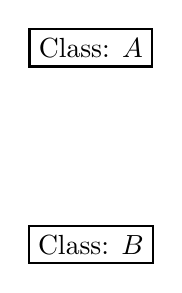
\begin{tikzpicture}[->, -latex, auto, node distance=2.5cm, thick, main node/.style={draw}]
                \node[main node] (1) {Class: $A$};
                \node[main node] (2) [below of=1] {Class: $B$};
            \end{tikzpicture}
        \end{adjustbox}
    \end{subfigure}
    \hfill
    \begin{subfigure}{.1\textwidth}
        \centering
        \huge{$\Longrightarrow$}
    \end{subfigure}
    \hfill
    \begin{subfigure}{.4\textwidth}
        \centering
        \begin{adjustbox}{valign=c, max width=\textwidth}
            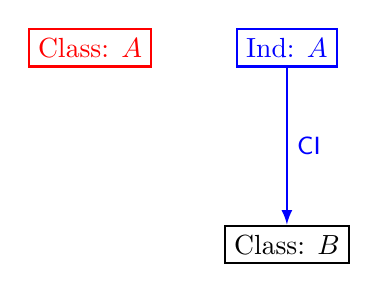
\begin{tikzpicture}[->, -latex, auto, node distance=2.5cm, thick, main node/.style={draw}]
                \node[main node] (1) [color=red] {Class: $A$};
                \node[main node] (2) [right of=1, color=blue] {Ind: $A$};
                \node[main node] (3) [below of=2] {Class: $B$};
                \path[every node/.style={font=\sffamily\small}]
                (2) edge [color=blue] node {CI} (3);
            \end{tikzpicture}
        \end{adjustbox}
    \end{subfigure}
    \caption{Exemple d'ajout du fait $CI(A,B)$}
    \label{fig:rule_ci}
\end{figure}

\gls{setup} donne priorité aux mises à jour, en définissant un ensemble d'effets de bord qui doivent être réalisés pour modifier la base afin de maintenir la cohérence après l'ajout d'un fait.
Les effets de bord sont un ensemble de règles de réécriture construit à partir des règles sémantiques de \gls{rdfs}.
\cite{chabinUsingGraphGrammar2019} propose différents niveaux de modification autorisés.
Ce niveau peut être paramétré pour chaque utilisateur lui donnant ainsi certains droits de modification.
Le niveau le plus élevé est autorisé à modifier le schéma et l'instance pour ajouter un fait.
Un niveau moins élevé permet seulement de modifier l'instance tandis que le niveau le plus bas ne peut pas modifier la base et peut donc seulement ajouter ou supprimer un fait si la cohérence de la base est maintenue.

\begin{figure}[htb]
    \begin{subfigure}{.45\textwidth}
        \begin{align}
            Cl(x) \label{eq:rule_csub:cl-x}\\
            Cl(y) \lor (y = Resource) \label{eq:rule_csub:cl-y}\\
            \neg CSub(y, x) \label{eq:rule_csub:not-csub}
        \end{align}
    \end{subfigure}
    \hfill
    \begin{subfigure}{.4\textwidth}
        \begin{align}
            \forall z ~ CSub(y, z) \to CSub(x, z) \label{eq:rule_csub:csub-bot}\\
            \forall z ~ CSub(z, x) \to CSub(z, y) \label{eq:rule_csub:csub-top}\\
            \forall z ~ CI(z, x) \to CI(z, y) \label{eq:rule_csub:ci}
        \end{align}
    \end{subfigure}
    \caption{Effets de bord pour l'ajout du fait $CSub(x, y)$}
    \label{eq:rule_csub}
\end{figure}

\begin{example}
    La figure~\ref{fig:app_rule} représente une base de connaissance initiale (en noir) et les modifications nécessaires (en bleu) pour l'ajout du fait $CSub(C_1, C_2)$.
    En suivant les effets de bord figure~\ref{eq:rule_csub}, l'ajout du fait $CSub(C_1, C_2)$ implique que $C_1$ et $C_2$ soient des classes par les effets de bord \ref{eq:rule_csub:cl-x} et \ref{eq:rule_csub:cl-y} respectivement.
    Comme $C_2$ n'est pas présent, le schéma doit être modifié.
    Le fait $CSub(C_2, Resource)$ est alors ajouté comme effet de bord de l'insertion de $Cl(C_2)$.
    Par la suite, le fait $CSub(C_1, C_2)$ peut être ajouté en ajoutant aussi le fait $CI(I, C_2)$ par transitivité de la relation $CI$ via l'effet de bord~\ref{eq:rule_csub:ci}.
    Cet exemple montre l'application d'effets de bord pour rendre applicable une règle.
    Sans ces effets de bord, il aurait été impossible d'ajouter le fait voulu tout en respectant les règles d'intégrité.
    Ici, l'individu $I$ est bien l'instance d'une classe et de toutes les sous-classes associées.
    La base avant et après application de la règle est un graphe \gls{rdfs} valide.
\end{example}

\begin{figure}[htb]
    \centering
    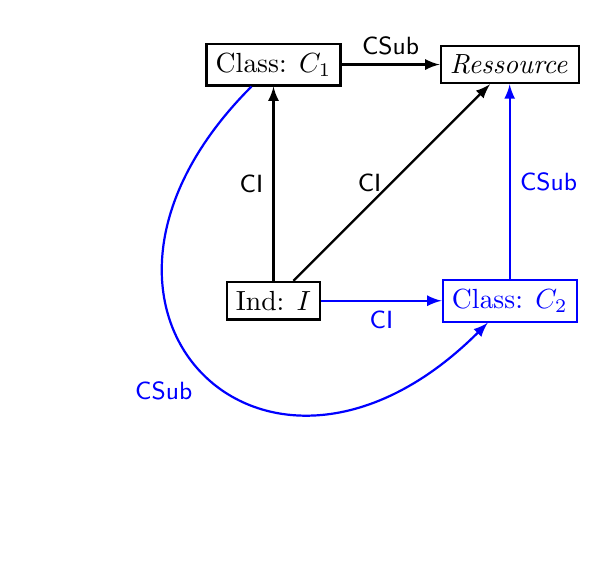
\begin{tikzpicture}[->, -latex, auto, node distance=3cm, thick, main node/.style={draw}]
        \node[main node] (1) {Ind: $I$};
        \node[main node] (2) [above of=1] {Class: $C_1$};
        \node[main node] (3) [right of=1, color=blue] {Class: $C_2$};
        \node[main node] (4) [above of=3] {\emph{Ressource}};
        \path[every node/.style={font=\sffamily\small}]
        (1) edge node [left] {CI} (2)
        (1) edge [color=blue] node [below] {CI} (3)
        (1) edge node [left] {CI} (4)
        (2) edge node [above] {CSub} (4)
        (2) edge [color=blue, distance=4cm, bend right=90] node [below left] {CSub} (3)
        (3) edge [color=blue] node [right] {CSub} (4);
    \end{tikzpicture}
    \vspace{-5em}
    \caption{Exemple de modification pour l'application d'une règle}
    \label{fig:app_rule}
\end{figure}

% Pour garantir la reproductibilité de ces travaux, l'implémentation du \gls{setup} est disponible en ligne dans un dépôt \gls{git} \cite{}.
% Ce dépôt contient également les jeux de données et le code nécessaires pour reproduire les benchmarks.

\gls{setup} fait partie du projet ANR \gls{sendup} \cite{ReSEauxNumeriquesDonnees,SENDUPSEmanticNetwork} qui vise à concevoir des mécanismes d'anonymisation pour les données structurées en graphes.
Plus précisément, \gls{sendup} se concentre sur les données \gls{rdf} et cherche à développer des approches pratiques, étayées par des modèles théoriques formels, pour garantir la confidentialité tout en préservant l'utilité des informations lors de la publication ou de l'interrogation de bases de données sous forme de graphes avec une sémantique sous-jacente.

\FloatBarrier
